\begin{figure}
    \centering
    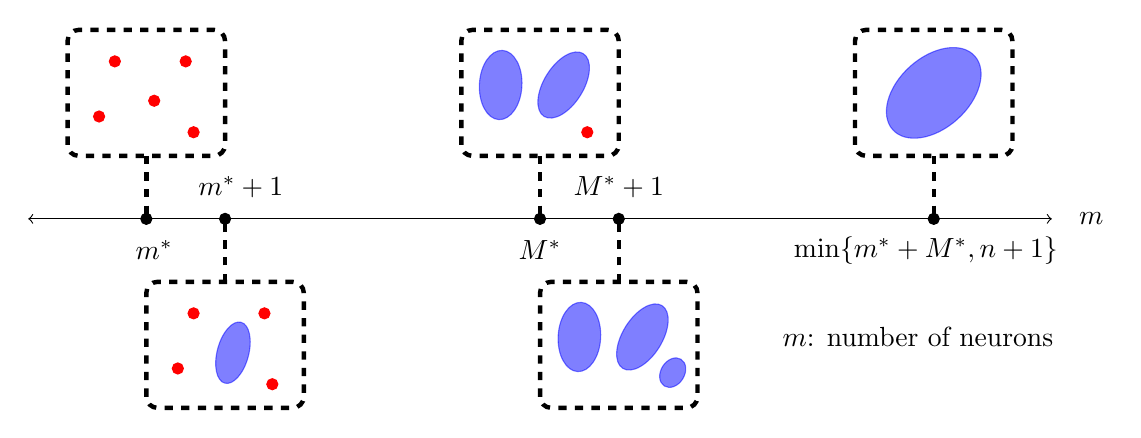
\begin{tikzpicture}{}
        \draw[<->] (-7,0) -- (6,0);
        \node at (-5.4,-0.4) {$m^{*}$};
        \node at (-4.3,0.4) {$m^{*}+1$};
        \node at (-0.5,-0.4) {$M^{*}$};
        \node at (0.5,0.4) {$M^{*}+1$};
        \node at (6.5,0) {$m$};
        \node at (4.3,-1.5) {$m$: number of neurons};
        \node at (4.4,-0.4) {$\min\{m^{*}+M^{*}, n+1\}$};
        \draw[fill=black] (-5.5,0) circle (2pt);
        \draw[fill=black] (-4.5,0) circle (2pt);
        \draw[fill=black] (-0.5,0) circle (2pt);
        \draw[fill=black] (0.5,0) circle (2pt);
        \draw[fill=black] (4.5,0) circle (2pt);
        \draw [draw=black,ultra thick,dashed,rounded corners] (-6.5,0.8) rectangle (-4.5,2.4);
        \draw[ultra thick, dashed] (-5.5,0.8) -- (-5.5,0);
        \draw [draw=black,ultra thick,dashed,rounded corners] (3.5,0.8) rectangle (5.5,2.4);
        \draw[ultra thick, dashed] (4.5,0.8) -- (4.5,0);
        \draw [draw=black,ultra thick,dashed,rounded corners] (-1.5,0.8) rectangle (0.5,2.4);
        \draw[ultra thick, dashed] (-0.5,0.8) -- (-0.5,0);
        \draw [draw=black,ultra thick,dashed,rounded corners] (-0.5,-2.4) rectangle (1.5,-0.8);
        \draw[ultra thick, dashed] (0.5,-0.8) -- (0.5,0);
        \draw [draw=black,ultra thick,dashed,rounded corners] (-5.5,-2.4) rectangle (-3.5,-0.8);
        e\draw[ultra thick, dashed] (-4.5,-0.8) -- (-4.5,0);

        \draw[fill=red,color = red] (-5.9,2) circle (2pt);
        \draw[fill=red,color = red] (-5.4,1.5) circle (2pt);
        \draw[fill=red,color = red] (-5,2) circle (2pt);
        \draw[fill=red,color = red] (-6.1,1.3) circle (2pt);
        \draw[fill=red,color = red] (-4.9,1.1) circle (2pt);

        \draw[fill=red,color = red] (-4.9,2-3.2) circle (2pt);
        \draw[fill=blue,color = blue, opacity = 0.5, rotate around={-15:(-4.4,-1.7)}] (-4.4,1.5-3.2) ellipse (0.2 and 0.4);
        \draw[fill=blue,color = red] (-4,2-3.2) circle (2pt);
        \draw[fill=red,color = red] (-5.1,1.3-3.2) circle (2pt);
        \draw[fill=red,color = red] (-3.9,1.1-3.2) circle (2pt);

        \draw[fill=blue,color = blue, opacity = 0.5, rotate around={-3:(-4.4+3.4,1.7)}] (-4.4+3.4,1.7) ellipse (0.27 and 0.44);
        \draw[fill=blue,color = blue, opacity = 0.5, rotate around={-32:(-4.4+4.2,1.7)}] (-4.4+4.2,1.7) ellipse (0.25 and 0.47);
        \draw[fill=red,color = red] (-3.9+4,1.1) circle (2pt);

        \draw[fill=blue,color = blue, opacity = 0.5, rotate around={-3:(-4.4+3.4+1,1.7-3.2)}] (-4.4+3.4+1,1.7-3.2) ellipse (0.27 and 0.44);
        \draw[fill=blue,color = blue, opacity = 0.5, rotate around={-32:(-4.4+4.2+1,1.7-3.2)}] (-4.4+4.2+1,1.7-3.2) ellipse (0.25 and 0.47);
        \draw[fill=blue,color = blue, opacity = 0.5, rotate around={-32:(-3.9+4+1,1.1-3)}] (-3.9+4.1+1,1.1-3) ellipse (0.15 and 0.2);
        \draw[fill=blue,color = blue, opacity = 0.5, rotate around={-48:(4.5,1.6)}] (4.5,1.6) ellipse (0.45 and 0.7);
    \end{tikzpicture}
\end{figure}
